\documentclass[11pt]{article}

\usepackage[a4paper,margin=2.4cm]{geometry}
\usepackage{amsmath,amssymb}
\usepackage{booktabs}
\usepackage{siunitx}
\usepackage{graphicx}
\usepackage[hidelinks]{hyperref}
\usepackage{enumitem}

\newcommand{\tirr}{t_{\mathrm{irr}}}
\newcommand{\tdel}{t_{\mathrm{del}}}
\newcommand{\tmeas}{t_{\mathrm{meas}}}
\newcommand{\file}[1]{\texttt{#1}}

\title{The scenario data product:\\
structure, metadata, and downstream use}
\author{Method note}
\date{\today}

\begin{document}
\maketitle

\begin{abstract}
A \emph{scenario} is the frozen output of one proton run (Stage~A) plus its
decay handoff (Stage~B0): a detector-independent positron-annihilation source
that a downstream PET simulation reads and turns into a measured acquisition.
This note specifies the scenario as a data product --- its files, their columns
and metadata, the shared coordinate frame, and the recipe a consumer follows to
build an acquisition from it --- so that a scenario directory can be used from
its own contents alone. The format is generic; the standard skull-base case
(\file{head\_sobp\_1e7}: a brain-filled head cylinder) is worked through as a
running example in Sec.~\ref{sec:example}. The physics behind the source is in
the user guide (\file{01\_user\_guide.tex}) and the decay bookkeeping in
\file{03\_decay\_kinetics.tex}; this note is the consumer-facing interface contract.
\end{abstract}

\section{What a scenario is}

The source side of the pipeline produces, once, a description of \emph{where}
$\beta^{+}$ emitters annihilate after a proton field irradiates a phantom. It is
deliberately \textbf{detector-independent}: it knows nothing about any ring,
crystal, or reconstruction. A scenario freezes one such run into a named
directory so that any number of detector studies can read the identical source.

A scenario carries three logically distinct pieces of information, plus
reference and provenance files:
\begin{description}[leftmargin=1.6em]
  \item[\emph{where}] the spatial source --- the annihilation points
    (\file{emitters.csv});
  \item[\emph{how many}] the measured decays per isotope at a chosen acquisition
    timing (\file{sampling\_budget\_<scenario>.csv});
  \item[\emph{through what}] the phantom medium the \SI{511}{keV} photons
    traverse (\file{phantom\_regions.csv} $+$ \file{phantom\_material\_*}).
\end{description}
The consumer combines these (Sec.~\ref{sec:use}). The split matters: the spatial
source is expensive and computed once; the number depends on dose and timing and
is a tiny separate file; the medium is implied by the run but not carried in the
point list, so it is materialized explicitly.

\section{Coordinate frame}
\label{sec:frame}

\begin{figure}[t]
  \centering
  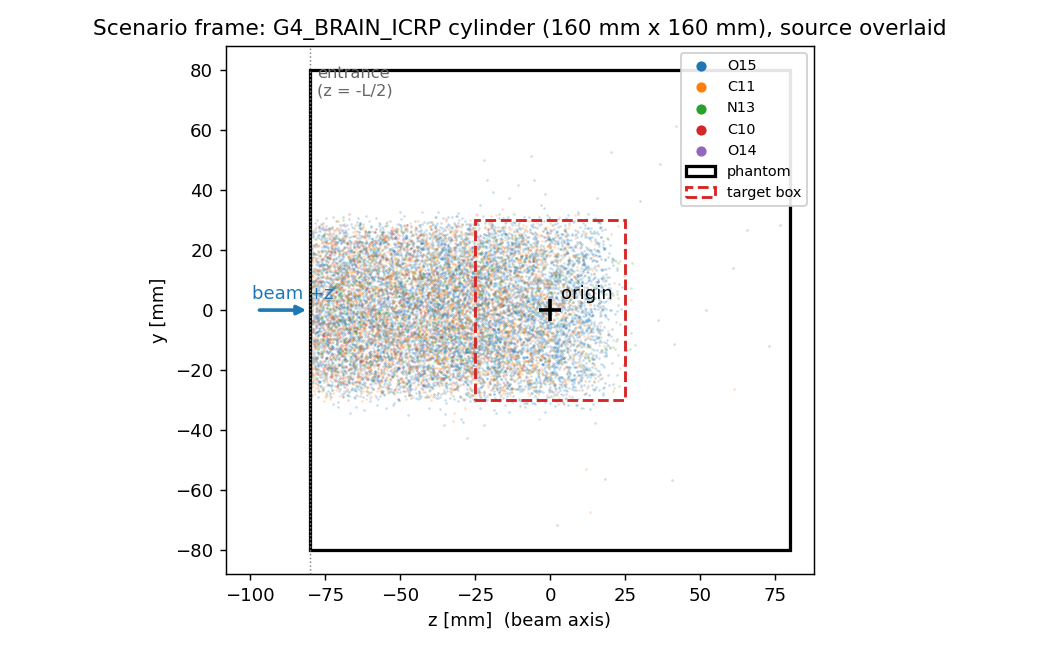
\includegraphics[width=\linewidth]{scenario_geometry.png}
  \caption{The scenario frame, drawn from \file{run\_meta.csv} with a subsample
  of \file{emitters.csv} annihilation points overlaid (one colour per isotope).
  The phantom is a cylinder centred at the origin with its axis along $+z$, the
  beam direction; the beam enters at the $z=-L/2$ face. The source cloud fills
  the proton path and tapers at the distal edge; it is laterally confined to the
  irradiated disk. The dashed box is the dose-normalisation target. This is the
  standard \file{head\_sobp\_1e7} case.}
  \label{fig:frame}
\end{figure}

All positions in a scenario --- the annihilation points, the phantom, and the
target box --- share \textbf{one Cartesian frame} (Fig.~\ref{fig:frame}):
\begin{itemize}[leftmargin=1.6em]
  \item The phantom is a cylinder \textbf{centred at the origin} with its axis
    along $+z$, the direction the proton beam travels.
  \item It spans $z\in[-L/2,\,+L/2]$ and radius $r=\sqrt{x^2+y^2}\in[0,R]$, with
    $L=\file{phantom\_length\_mm}$ and $R=\file{phantom\_diameter\_mm}/2$.
  \item The beam enters at the $z=-L/2$ face. Depth into the phantom, measured
    from that face, is
    \begin{equation}
      d = z + L/2, \qquad\text{equivalently}\qquad z = d - L/2 .
      \label{eq:depth}
    \end{equation}
    The target-box depths in \file{run\_meta.csv} are measured from the
    entrance, so they map to $z=\file{target\_*\_depth\_mm}-L/2$.
\end{itemize}
A consumer that instantiates the phantom with its centre at the origin is
co-registered with the \file{emitters.csv} source: no offset or rotation is
needed.

\section{File reference}
\label{sec:files}

Units throughout: position \si{mm}, energy \si{keV} (beam energy \si{MeV}), time
\si{s} for acquisition timing, dose \si{Gy}. Each data file with run-level
scalars has a companion \file{*\_meta.csv} (a single wide row). The terse
machine copy of this reference ships inside every scenario as \file{SCHEMA.md};
this section is its canonical, annotated form.

\subsection{\file{emitters.csv} --- the spatial source}

One row per produced $\beta^{+}$ emitter; the high-statistics production shape.

\begin{center}
\begin{tabular}{@{}lll@{}}
\toprule
column & type & meaning \\
\midrule
\file{event\_id} & int & primary proton that produced it (diagnostic) \\
\file{isotope\_id} & int8 & isotope code (see \file{isotopes.csv}) \\
\file{prod\_x\_mm}, \file{prod\_y\_mm}, \file{prod\_z\_mm} & float & production point --- the truth map \\
\file{anh\_x\_mm}, \file{anh\_y\_mm}, \file{anh\_z\_mm} & float & annihilation point --- the detector source \\
\bottomrule
\end{tabular}
\end{center}

The positron range per emitter is $\file{anh}-\file{prod}$. Positrons that would
leave the phantom into air are stopped at the surface, so a small fraction
($\sim$\SI{0.6}{\percent}) have their \file{anh} pinned to the boundary. The
file holds the production \emph{shape} at the simulated statistics; the absolute
measured count is set by the budget, never here.

\subsection{\file{run\_meta.csv} --- run-level metadata}

One wide row. Beam, geometry, dosimetry, and provenance.

\begin{center}
\begin{tabular}{@{}lll@{}}
\toprule
column & type & meaning \\
\midrule
\file{n\_protons} & int & primaries simulated \\
\file{beam\_energy\_MeV} & float & nominal proton energy; for a SOBP run, the \\
 & & fallback single energy (real spectrum in \file{sobp\_layers.csv}) \\
\file{beam\_sigma\_mm} & float & Gaussian beam $\sigma$ at entrance (pencil mode) \\
\file{phantom\_material} & string & Geant4 NIST name, e.g.\ \file{G4\_BRAIN\_ICRP} \\
\file{phantom\_diameter\_mm}, \file{phantom\_length\_mm} & float & phantom cylinder size \\
\file{phantom\_mass\_g} & float & phantom mass \\
\file{edep\_total\_MeV} & float & total energy deposited in the phantom \\
\file{dose\_total\_Gy} & float & whole-phantom dose for \file{n\_protons} \\
\file{target\_dose\_Gy} & float & dose in the target box for \file{n\_protons} \\
\file{target\_mass\_g} & float & target-box mass \\
\file{target\_radius\_mm} & float & target box (cylinder) radius \\
\file{target\_prox\_depth\_mm}, \file{target\_dist\_depth\_mm} & float & target faces, depth from entrance \\
\file{Np\_per\_Gy} & float & protons for \SI{1}{Gy} ($=\file{n\_protons}/\file{target\_dose\_Gy}$) \\
\file{geant4\_version}, \file{physics\_list}, \file{random\_seed} & & provenance \\
\bottomrule
\end{tabular}
\end{center}

The absolute normalization scales production to a clinical dose $D$ via
\file{target\_dose\_Gy}: $P_j(D)=\file{count}_j\cdot D/\file{target\_dose\_Gy}$.

\subsection{\file{sampling\_budget\_<scenario>.csv} --- measured decays}

One row per isotope. The thin quantity the handoff hands across to the detector
study.

\begin{center}
\begin{tabular}{@{}lll@{}}
\toprule
column & type & meaning \\
\midrule
\file{isotope\_id} & int8 & isotope code \\
\file{N\_expected} & float & expected measured decays for \SI{1}{Gy} at this timing \\
\bottomrule
\end{tabular}
\end{center}

The companion \file{*\_meta.csv} carries \file{scenario}, \file{source\_file},
\file{dose\_Gy}, and the acquisition timing \file{t\_irr\_s}, \file{t\_del\_s},
\file{t\_meas\_s}. The measured decays follow the three-factor expression
(\file{03\_decay\_kinetics.tex}, Eq.~1)
\begin{equation}
  N_j = P_j(D)\cdot
        \underbrace{\frac{1-e^{-\lambda_j \tirr}}{\lambda_j \tirr}}_{\text{build-up}}\cdot
        \underbrace{e^{-\lambda_j \tdel}}_{\text{transport}}\cdot
        \underbrace{\bigl(1-e^{-\lambda_j \tmeas}\bigr)}_{\text{window}} .
  \label{eq:budget}
\end{equation}
A scenario may carry several budgets that differ \emph{only} in timing; the
spatial source is shared. The standard set: \file{inroom} (baseline,
$\tdel=\SI{120}{s}$), \file{fast} ($\tdel=\SI{60}{s}$), and \file{offline}
($\tdel=\SI{300}{s}$, $\tmeas=\SI{1800}{s}$). Shorter delay keeps more
short-lived $^{15}$O.

\subsection{\file{phantom\_regions.csv} $+$ \file{phantom\_material\_*} --- the medium}

The source is detector-independent but \textbf{not} medium-independent: a PET
simulation must propagate the \SI{511}{keV} annihilation photons through the
phantom and needs the material at each point (for attenuation $+$ scatter, and
$\mu$ for reconstruction attenuation correction). The medium is two files:

\textbf{\file{phantom\_regions.csv}} --- \emph{where} each material is: one row
per region, in the same world frame as \file{emitters.csv}, with
\file{region}, \file{priority}, \file{material}, \file{solid}
(\file{ellipsoid}/\file{cylinder}), semi-axes \file{a\_mm,b\_mm,c\_mm} (cylinder:
$r,r,\text{half-length}$), centre \file{cx\_mm,cy\_mm,cz\_mm}, and Euler angles
\file{euler\_\{x,y,z\}\_deg}. The regions are \textbf{axis-aligned} (Euler angles
$0$); a point takes the material of the first (lowest-\file{priority}) region
containing it, else air, with ellipsoid membership
$((x-c_x)/a)^2+((y-c_y)/b)^2+((z-c_z)/c)^2\le 1$. Brain-first ordering carves the
skull shell, so no boolean solids are needed. The cylinder writes one row; the
MIRD head writes brain/skull/scalp.

\textbf{\file{phantom\_material\_<material>.csv}} --- \emph{what} each material
is: one per distinct material in \file{phantom\_regions.csv}. The composition
file has one row per element (\file{element}, \file{Z}, \file{A\_g\_mol},
\file{mass\_fraction}); the companion \file{*\_meta.csv} carries
\file{density\_g\_cm3}, \file{mean\_excitation\_eV}, $\mu/\rho$
(\file{mu\_rho\_cm2\_g}) and $\mu$ (\file{mu\_cm\_inv}) at \file{energy\_keV}$=511$,
and \file{mean\_free\_path\_cm}. Compositions are the authoritative Geant4 NIST
definitions; $\mu$ is Compton/Klein--Nishina (coherent $+$ photoelectric,
$\sim$1--\SI{2}{\percent} at \SI{511}{keV}, are not included). This covers
homogeneous (one region) and analytic multi-region (e.g.\ the MIRD head)
phantoms; a fully \emph{voxelized} patient would instead need a voxel map and is
deferred.

\subsection{Reference and figures}

\file{isotopes.csv} decodes \file{isotope\_id}: \file{name},
\file{half\_life\_s}, \file{endpoint\_MeV}, and \file{prompt\_gamma} (1 if the
isotope emits a prompt de-excitation $\gamma$ in coincidence --- relevant to PET
backgrounds). \file{sobp\_layers.csv} is the beam definition (energy layers and
weights). \file{SCHEMA.md} is the terse column reference; \file{README.md} is the
scenario writeup with numbers filled in. \file{figures/} holds the realized
depth-dose, the Stage-A validation dashboard, and the activity curves.

\section{How a consumer builds an acquisition}
\label{sec:use}

The scenario gives the source; the detector study realizes it. The recipe:
\begin{enumerate}[leftmargin=1.8em]
  \item Choose a timing budget and read $N_{\mathrm{expected},j}$ per isotope
    from \file{sampling\_budget\_<scenario>.csv}. (Rescale linearly for a dose
    other than \SI{1}{Gy}.)
  \item For each isotope $j$, draw $M_j\sim\mathrm{Poisson}(N_{\mathrm{expected},j})$
    annihilation points by sampling, with replacement, the rows of
    \file{emitters.csv} with that \file{isotope\_id} (columns
    \file{anh\_x/y/z\_mm}). Seed reproducibly --- e.g.\
    $\text{master\_seed}+\text{realization}$ --- so every detector configuration
    sees the \emph{identical} source.
  \item From each sampled point, emit a back-to-back \SI{511}{keV} photon pair
    (isotropic direction, with the chosen non-collinearity blur).
  \item Transport the photons through the phantom defined by
    \file{phantom\_regions.csv} (region $\to$ material at each point) and
    \file{phantom\_material\_*} (its $\mu$); use the same medium for
    reconstruction attenuation correction.
\end{enumerate}
All randomness (the Poisson draw, the emission directions) lives in the consumer;
the scenario itself is deterministic and seed-free, so the source is reproducible
across studies. The spread of the recovered proton range over realizations,
$\sigma(\text{range})$, is the figure of merit (\file{03\_decay\_kinetics.tex}).

\section{Worked example: \file{head\_sobp\_1e7}}
\label{sec:example}

The standard skull-base reference: a proton SOBP field delivering \SI{1}{Gy} to
a target inside a head, modelled as a homogeneous brain cylinder. It is the case
drawn in Fig.~\ref{fig:frame}.

\paragraph{Geometry and beam.} A \file{G4\_BRAIN\_ICRP} cylinder,
\SI{160}{mm} diameter $\times$ \SI{160}{mm} ($L=\SI{160}{mm}$, $R=\SI{80}{mm}$,
so $z\in[-80,80]\,$\si{mm}). The beam enters at $z=-\SI{80}{mm}$ and travels
$+z$; it is a spread-out Bragg peak (layers in \file{sobp\_layers.csv}) painted
over a uniform disk. The dose-normalisation target box is
\SI{60}{mm} diameter $\times$ \SI{50}{mm}, at \SI{55}{}--\SI{105}{mm} depth ---
by Eq.~\eqref{eq:depth}, $z\in[-25,25]\,$\si{mm} (the dashed box in
Fig.~\ref{fig:frame}). $10^{7}$ protons, Geant4~11.4.1, \file{QGSP\_BIC\_HP}.

\paragraph{Normalization.} The simulated target dose is
$\file{target\_dose\_Gy}\approx\num{5.97e-4}$ for $10^{7}$ protons, so reaching
\SI{1}{Gy} needs $\file{Np\_per\_Gy}\approx\num{1.68e10}$ protons; production
counts scale by that factor.

\paragraph{Source.} Per \SI{1}{Gy}, the integral yields are
$^{15}$O $\approx\num{2.5e8}$, $^{11}$C $\approx\num{1.1e8}$,
$^{13}$N $\approx\num{1.9e7}$, $^{10}$C $\approx\num{1.2e7}$,
$^{14}$O $\approx\num{8.7e6}$ (total $\approx\num{4e8}$), about
$2.2\times$ the Parodi~2008 Table~2 head values --- the expected level of
agreement for a Geant4 cross-section model on a homogeneous brain phantom.

\paragraph{Measured decays (in-room baseline).} Applying Eq.~\eqref{eq:budget} at
$\tirr=\SI{60}{}$, $\tdel=\SI{120}{}$, $\tmeas=\SI{1200}{s}$ gives
$N_{^{15}\mathrm O}\approx\num{1.07e8}$, $N_{^{11}\mathrm C}\approx\num{5.0e7}$
(total $\approx\num{1.7e8}$), a measured $^{15}$O$/^{11}$C $\approx 2.1$. The
\file{fast} budget ($\tdel=\SI{60}{s}$) raises that ratio to $\approx 2.9$; the
\file{offline} budget ($\tdel=\SI{300}{s}$) lowers it toward the Parodi
$\approx1.2$.

\paragraph{Medium.} \file{G4\_BRAIN\_ICRP}: $\rho=\SI{1.040}{g/cm^3}$, oxygen
mass fraction $0.712$, with $\mu/\rho=\SI{0.0953}{cm^2/g}$ and
$\mu=\SI{0.0991}{cm^{-1}}$ at \SI{511}{keV} (mean free path \SI{10.1}{cm}) ---
the attenuation a consumer applies to the back-to-back photons and in
reconstruction.

\paragraph{Building the acquisition.} Following Sec.~\ref{sec:use}: pick
\file{inroom}; draw $\sim\num{1.07e8}$ $^{15}$O and $\sim\num{5e7}$ $^{11}$C
annihilation points (and the rest) from \file{emitters.csv}; emit \SI{511}{keV}
pairs; transport through the brain cylinder above. The result is one Poisson
realization of the measured PET source for this field.

\end{document}
